
\section{Introduction}
\label{s:secIntro2HDM}
As described in Section~\ref{s:meritSM}, although the predictions of the SM 
match well with the experimental observation, the SM has no explanation
to many other observed phenomena. To be able to explain such phenomena, 
many extensions of the SM have been proposed. One of the simplest
extensions is the two Higgs doublet model (2HDM) where an extra Higgs doublet is
added to Equation~(\ref{eq:smLag}). In Lagrangian of the SM, there is only one Higgs SU(2) 
doublet comprising four Higgs fields. After the spontaneous symmetry breaking, 
only one Higgs ($h$) remains in the model as the other three Higgses are eaten 
away by the three gauge bosons ($W^\pm, ~Z$). In the 2HDM, there are two SU(2) 
Higgs doublets comprising eight Higgs fields. Three of them are again 
eaten away by the gauge bosons and the five Higgses ($h, H, A, H^\pm$) remains 
in the model. Further, the 2HDM is divided into four types (I, II, X, Y) based 
on the coupling of quarks and leptons with the two Higgs doublets. The type II
of the 2HDM corresponds to the MSSM (minimal supersymmetric extension of the 
standard model).
% in the limit where the mass of each particle is decoupled on a very large scale.

\section{The Higgs sector}
The Higgs potential term for the 2HDM is constructed in such a way so that it is 
invariant under Z$_2$ symmetry, where the Higgs doublets transform as 
$\Phi_1 \rightarrow \Phi_1, ~ \Phi_2 \rightarrow \text{-} \Phi_2$. The Z$_2$ symmetry
is imposed to avoid the flavor changing neutral currents (FCNC). The CP-conserving 
potential is given by \cite{PhysRevD.80.015017}
\begin{align}
V^\text{2HDM}
&= m_1^2\Phi_1^\dag\Phi_1+m_2^2\Phi_2^\dag\Phi_2
-m_3^2\left(\Phi_1^\dag\Phi_2+\Phi_2^\dag\Phi_1\right)
+\frac{\lambda_1}2(\Phi_1^\dag\Phi_1)^2
+\frac{\lambda_2}2(\Phi_2^\dag\Phi_2)^2\nonumber \\
&\qquad+\lambda_3(\Phi_1^\dag\Phi_1)(\Phi_2^\dag\Phi_2)
+\lambda_4(\Phi_1^\dag\Phi_2)(\Phi_2^\dag\Phi_1)
+\frac{\lambda_5}2\left[(\Phi_1^\dag\Phi_2)^2
+(\Phi_2^\dag\Phi_1)^2\right], 
\label{eq:pot2HDM}
\end{align}
where $m_i$ and $\lambda_i$ are scalar potential parameters taken to be real. 
The parameters are chosen such that the potential admits spontaneous symmetry breaking. Let $v_i$ be
the vacuum expectation value (vev) of the Higgs field $\Phi_i$. We expand
the Higgs field around its vev~\cite{PhysRevD.80.015017}, such that,

\begin{align}
\Phi_i=\begin{pmatrix}\omega_i^+\\\frac1{\sqrt2}(v_i+h_i-i\,z_i)
\end{pmatrix}.
\label{eq:higgs2HDM}
\end{align}
After substituting new fields from Equation (\ref{eq:higgs2HDM}) into (\ref{eq:pot2HDM}), 
one can see that there are off-diagonal terms for 
$\omega_i^+, ~ h_i, ~z_i$ fields. To remove these off-diagonal terms from the 
potential, these fields are reparametrized in terms of new fields $\omega^\pm, 
~H^+, ~z, ~A, ~h,$ and $H$ by using the following transformations \cite{PhysRevD.80.015017}
\begin{align}
\begin{pmatrix}h_1\\h_2\end{pmatrix}=\text{R}(\alpha)
\begin{pmatrix}H\\h\end{pmatrix},\quad
\begin{pmatrix}z_1\\z_2\end{pmatrix}=\text{R}(\beta)
\begin{pmatrix}z\\A\end{pmatrix},\quad
\begin{pmatrix}\omega_1^+\\\omega_2^+\end{pmatrix}=\text{R}(\beta)
\begin{pmatrix}\omega^+\\H^+\end{pmatrix},
\end{align}
where $R(\alpha), ~R(\beta)$ are the rotation matrices given by 
\cite{PhysRevD.80.015017}
\begin{align}
\text{R}(\theta)=\begin{pmatrix}\cos\theta&-\sin\theta\\
\sin\theta&\cos\theta\end{pmatrix}.
\end{align}
After the Higgs mechanism, the three Higgses are eliminated from the potential 
terms. They are eaten away by the three gauge bosons ($W^\pm, ~Z$). The free 
parameters in the potential are masses of the remaining five Higgses, $m_3^2$, 
$v$, $\tan\beta$, and $\cos(\beta -\alpha)$, where $v = \sqrt{v_1^2 + v_2^2}$ and 
$\tan\beta = v_1/v_2$. The scalar parameters in the potential and the physical parameters are 
listed in Table~\ref{tab:param2HDM}. 
%At tree level, only two physical parameters ($\tan\beta, ~m_A$) are independent, 
%the rest can be expressed in terms of these two.
\begin{table}
\begin{centering}
\caption{The scalar potential and physical parameters of the Higgs sector of the 2HDM.}
\label{tab:param2HDM}
\begin{tabular}{cc}
	\hline \noalign{\vskip 0.2cm}
	Scalar potential parameters & $m_1, ~m_2, ~m_3, ~\lambda_1, ~\lambda_2, ~\lambda_3,
	~\lambda_4, ~\lambda_5$\\ \noalign{\vskip 0.2cm}
	Physical parameters & $m_h^2, ~m_H^2, ~m_{H^\pm}^2 ~m_A^2, ~m_3^2, ~v, 
	~\tan\beta, ~\cos(\beta-\alpha)$ \\ \noalign{\vskip 0.2cm}
	\hline
	\end{tabular}
	\par\end{centering}
\end{table}

\section{The Yukawa sector}
The Yukawa sector of the 2HDM is considerably more complicated in comparison to that
of a single Higgs doublet. The general Lagrangian free from FCNC for the Yukawa sector is 
given as
%\begin{align}
%{\mathcal L}_\text{yukawa}^\text{2HDM} =
%&-{\overline Q}_LY_u\widetilde{\Phi}_uu_R^{}
%-{\overline Q}_LY_d\Phi_dd_R^{}
%-{\overline L}_LY_\ell\Phi_\ell \ell_R^{}+\text{H.c.},
%\label{eq:lagYu2HDM}
%\end{align}
\begin{equation}
\mathcal{L}_\text{Yukawa}^\text{2HDM} =  G^l\bar L \varphi_i R + G^d \bar{q_L} \varphi_i d_R +G^u \bar{q_L} \varphi_i^c u_R + h.c.,
\label{eq:lagYu2HDM}
\end{equation}
where $i$ can be 1 or 2. The interactions of the two Higgs doublets are different for different 
flavors of the fermions. Based on the different types of interaction, the 
2HDM is divided into four types as shown in Table~\ref{tab:type2HDM}. For example,
in Type II, the up-type quarks interact with the second Higgs doublet ($\varphi_2$), down 
type-quarks and leptons interact with the first Higgs doublet ($\varphi_1$).
\begin{table} 
\begin{centering} 
\caption{The different types of 2HDM. The quarks and leptons interact either
	with the first or the second Higgs doublet in different types.}
\label{tab:type2HDM} 
\begin{tabular}{ccccc} 
\hline 
\hline 
Coupling of &\textbf{Type-I} &\textbf{Type-II} &\textbf{Type-X} &\textbf{Type-Y}
\\ 
\hline 
\hline
\noalign{\vskip 0.1cm}
up-type quarks 	& $\Phi_2$  & $\Phi_2$ & $\Phi_2$ & $\Phi_1$ \\ 
\noalign{\vskip 0.1cm}                                                     
down-type quarks 	& $\Phi_2$  & $\Phi_1$ & $\Phi_2$ & $\Phi_2$ \\ 
\noalign{\vskip 0.1cm}                                                     
leptons 		& $\Phi_2$  & $\Phi_1$ & $\Phi_1$ & $\Phi_2$ \\ 
\noalign{\vskip 0.1cm}
\hline 
\end{tabular} 
\par\end{centering} 
\end{table}

The general form of the Lagrangian, as given by Equation (\ref{eq:lagYu2HDM}),
for all types of the 2HDM can be written as \cite{PhysRevD.80.015017}
\begin{align}
{\mathcal L}_\text{yukawa}^\text{2HDM} =
&-\sum_{f=u,d,\ell} \left( \frac{m_f}{v}G_h^f{\overline
f}fh+\frac{m_f}{v}G_H^f{\overline
f}fH-i\frac{m_f}{v}G_A^f{\overline f}\gamma_5fA\right)\nonumber\\
&-\left\{\frac{\sqrt2V_{ud}}{v}\overline{u}
\left(m_uG_A^u\text{P}_L+m_dG_A^d\text{P}_R\right)d\,H^+
+\frac{\sqrt2m_\ell G_A^\ell}{v}\overline{\nu_L^{}}\ell_R^{}H^+
+\text{H.c.}\right\},\label{Eq:Yukawa}
\end{align}
where $f$ is the fermion, $G^f_h$ is the coupling of fermion $f$ with the Higgs
boson $h$, and $P_{L/R}$ are projection operators. The value of $G^f$ is 
different for different types of the 2HDM as shown in Table~\ref{tab:coupling2HDM}. 
Only couplings with the Higgs $A$ is shown in this table
as only that is needed for the study of branching ratios of the charged Higgs boson.
Couplings of fermions with all the Higgses are given in \cite{PhysRevD.80.015017}
. The branching ratio of \PQt quark decays and the charged Higgs decays have been 
given in the next sections.
\begin{table} 
\begin{centering} 
\caption{The coupling of quarks and leptons with Higgs $A$ for all types of 2HDM.}
\begin{tabular}{ccccc} 
\hline 
\hline 
Coupling & Type-I & Type-II & Type-X & Type-Y \\ 
\hline 
\hline
\noalign{\vskip 0.1cm}
$G^u_A$ & $\cot\beta$  & $\cot\beta$ & $\cot\beta$ & $\cot\beta$ \\ 
\noalign{\vskip 0.1cm}
$G^d_A$ & $-\cot\beta$  & $\tan\beta$ & $-\cot\beta$ & $\tan\beta$ \\ 
\noalign{\vskip 0.1cm}
$G^l_A$ & $-\cot\beta$  & $\tan\beta$ & $\tan\beta$ & $-\cot\beta$ \\ 
\noalign{\vskip 0.1cm}
\hline 
\end{tabular} 
\par\end{centering} 
\label{tab:coupling2HDM} 
\end{table}


%\begin{figure}
%\begin{center}
%\begin{minipage}{0.24\hsize}
%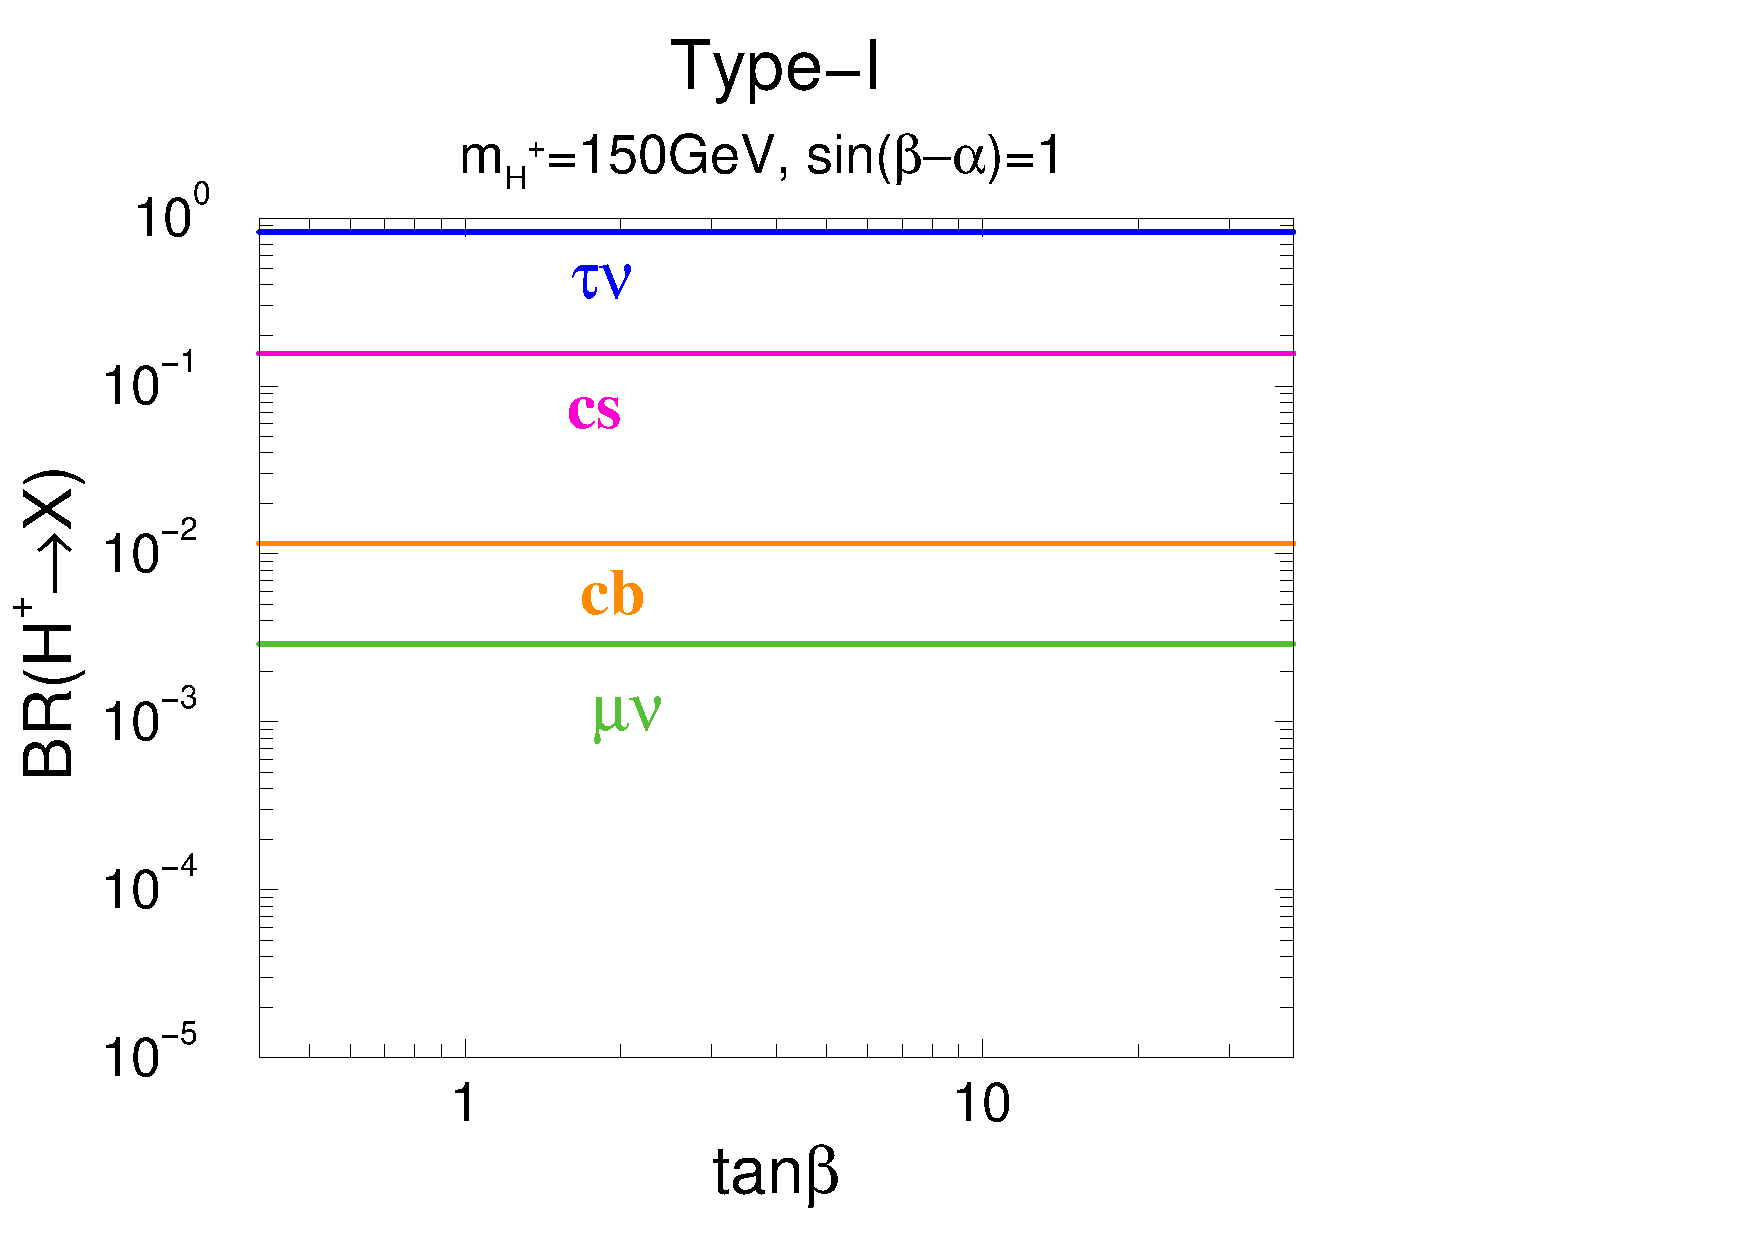
\includegraphics[width=1.7\linewidth]{Theory/Image/BR_ch_1.pdf}
%\end{minipage}
%\begin{minipage}{0.24\hsize}
%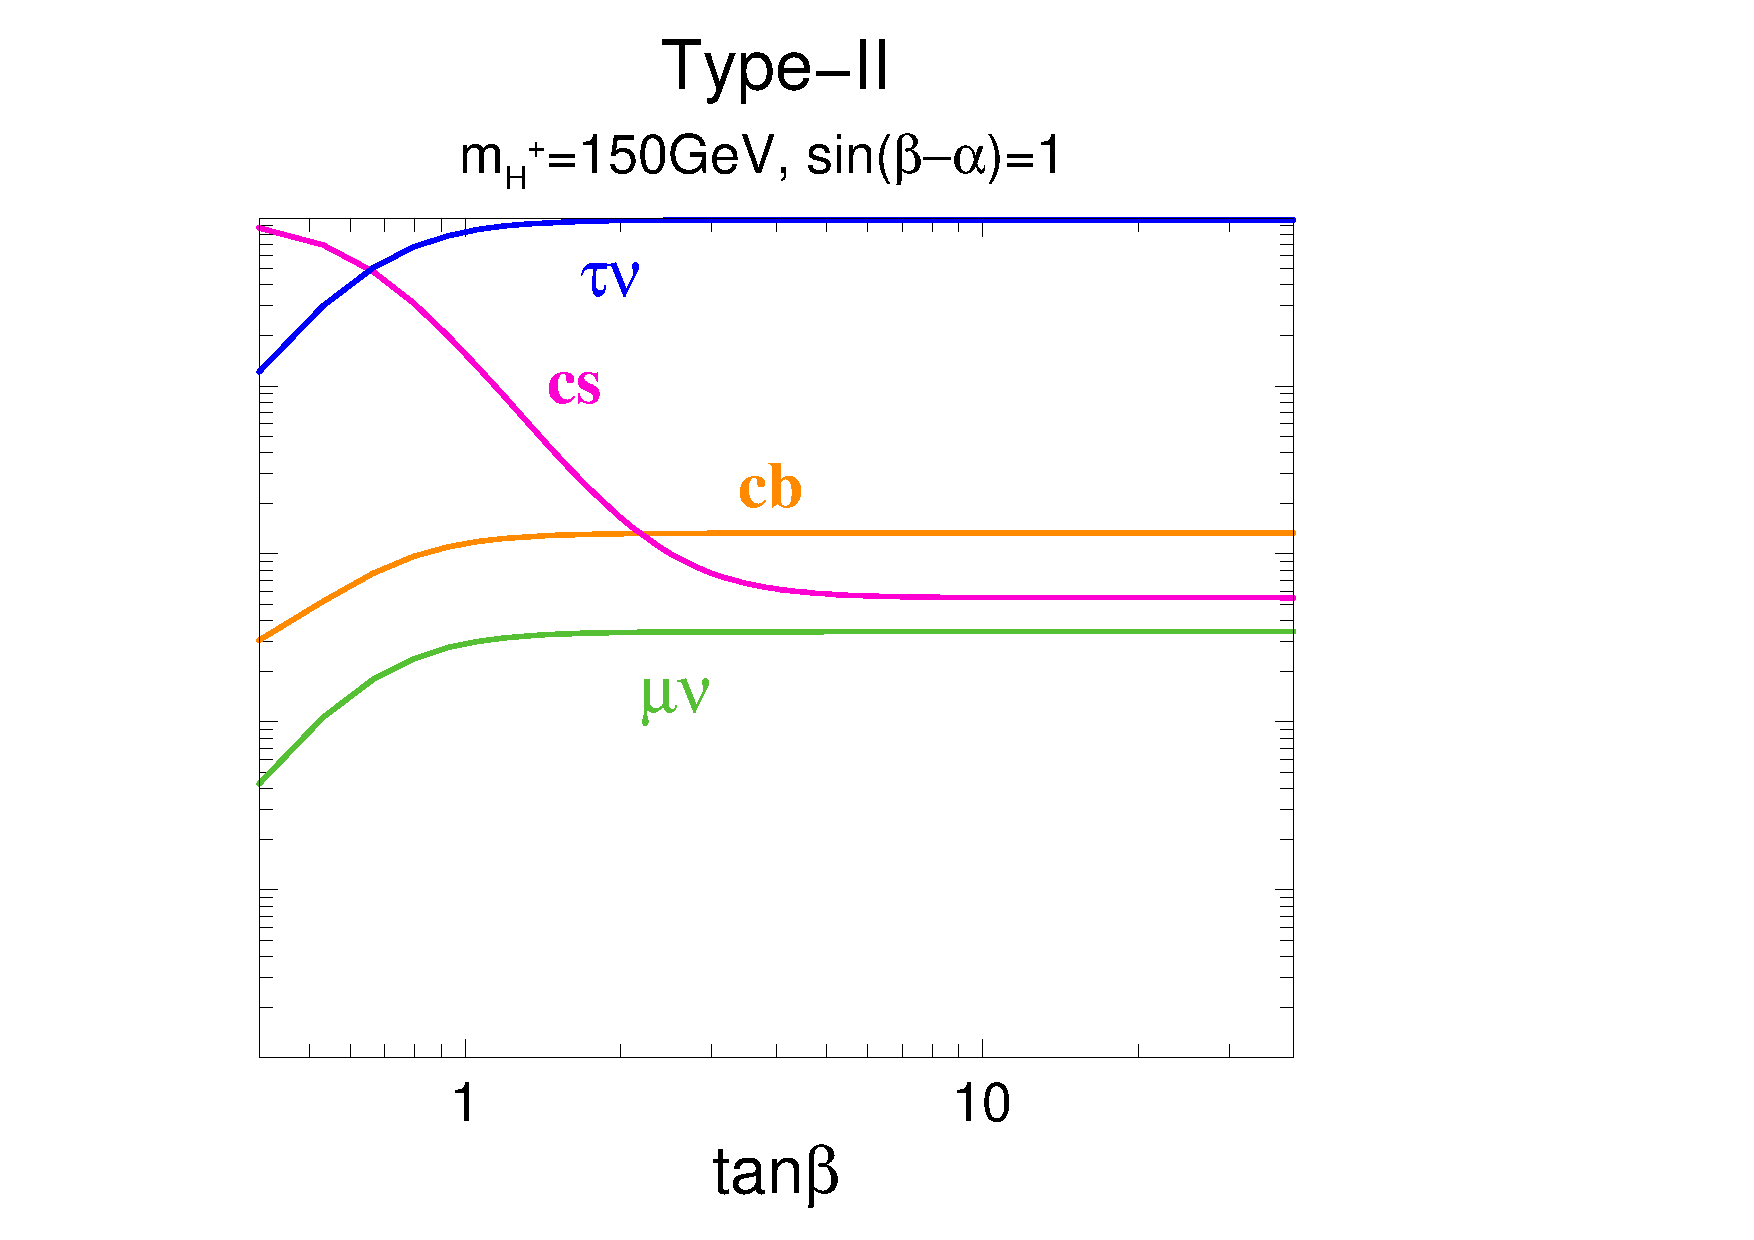
\includegraphics[width=1.7\linewidth]{Theory/Image/BR_ch_2.pdf}
%\end{minipage}
%\begin{minipage}{0.24\hsize}
%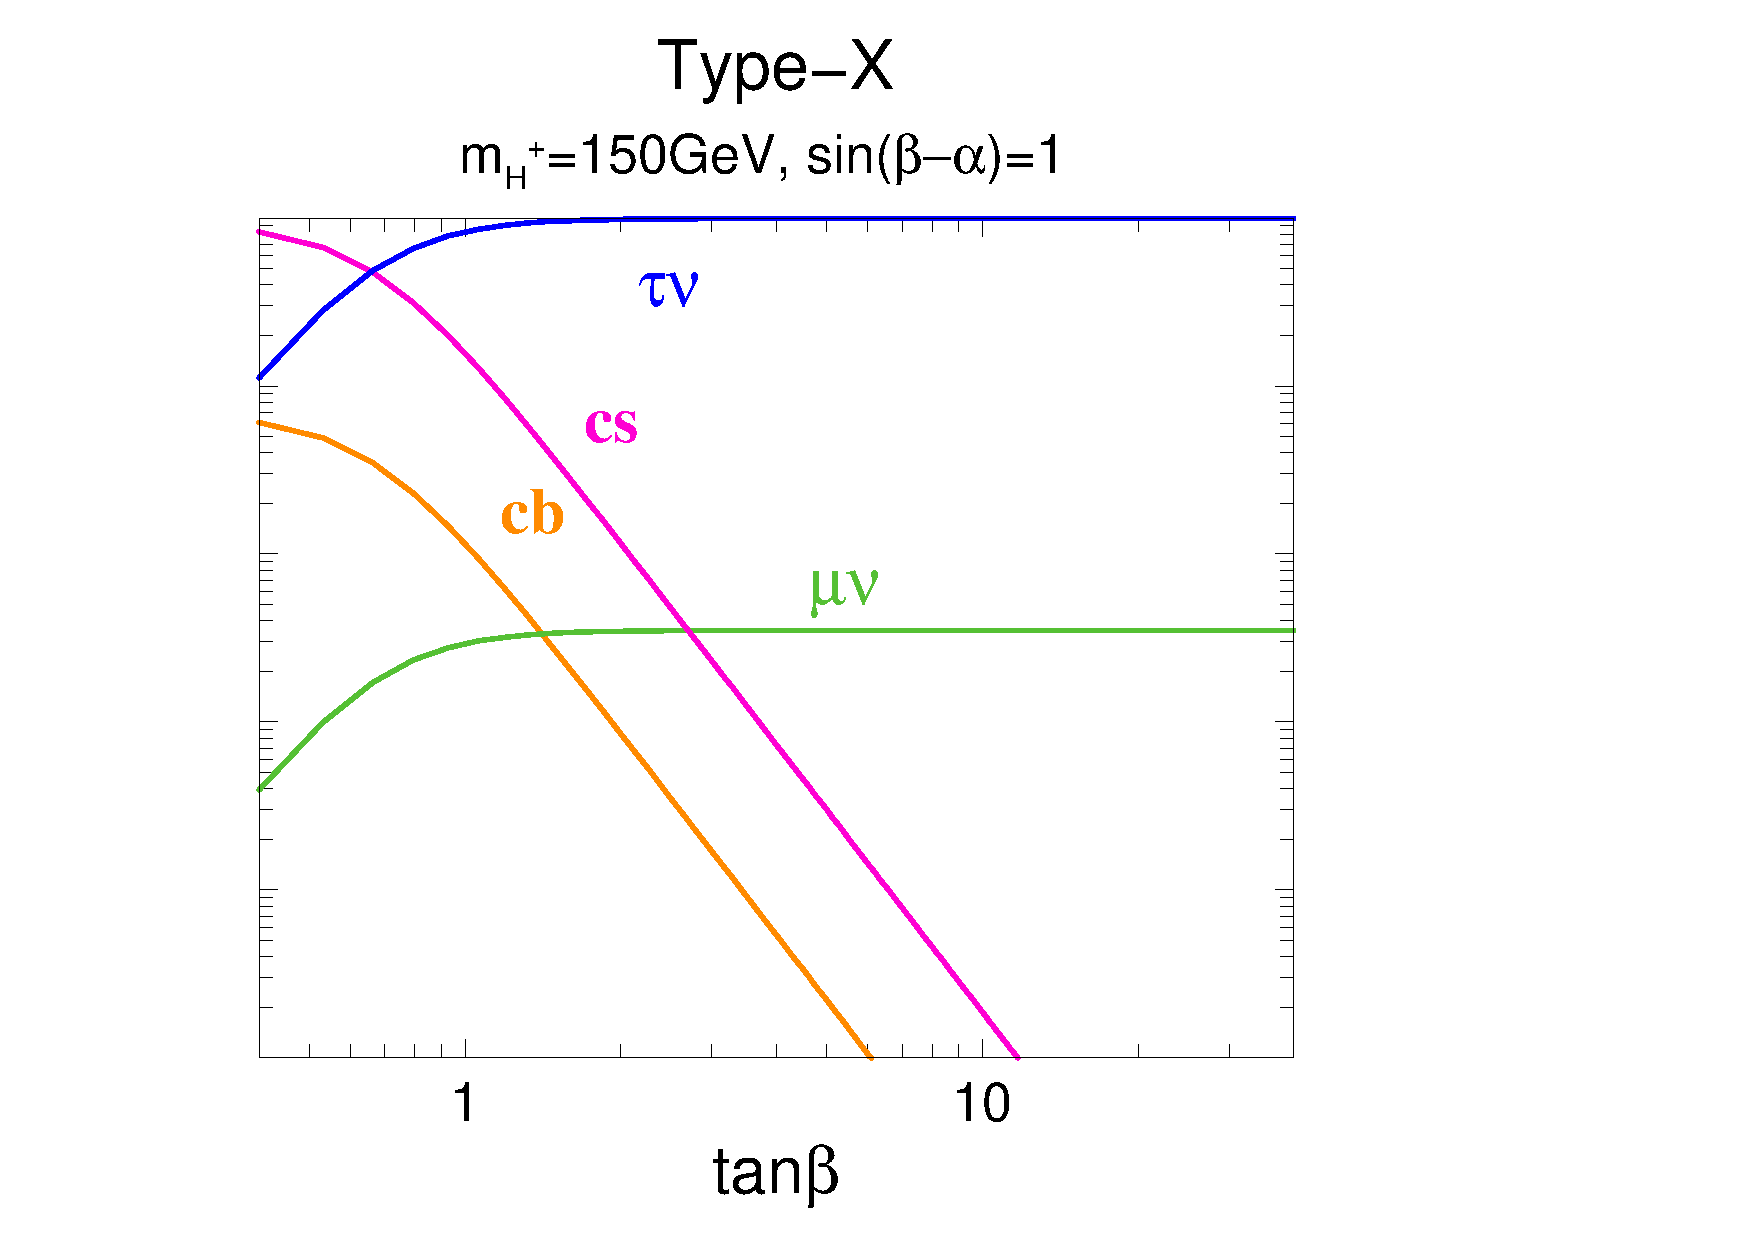
\includegraphics[width=1.7\linewidth]{Theory/Image/BR_ch_X.pdf}
%\end{minipage}
%\begin{minipage}{0.24\hsize}
%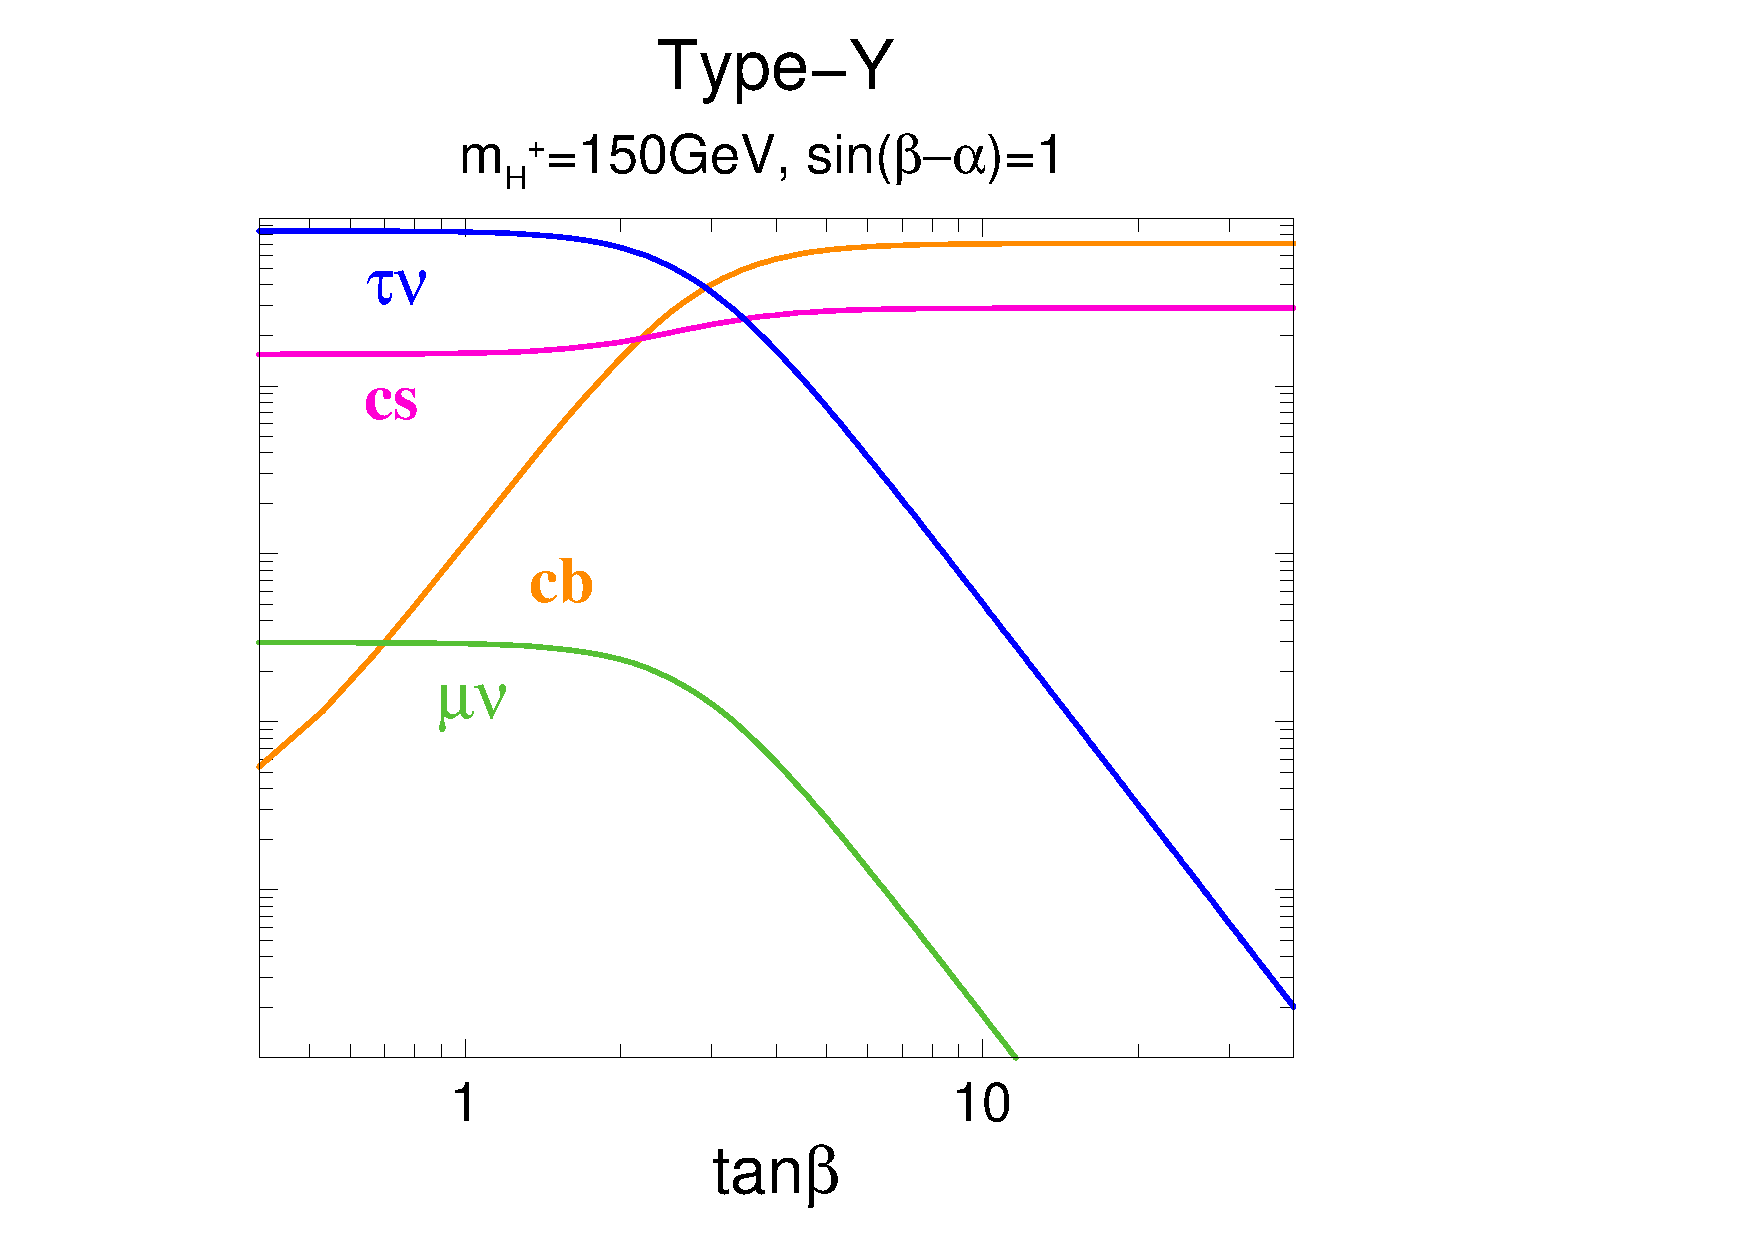
\includegraphics[width=1.7\linewidth]{Theory/Image/BR_ch_Y.pdf}
%\end{minipage}
%\caption{Decay branching ratios of $H$, $A$ and $H^\pm$
%in the four different types of THDM as a function of $\tan\beta$
%for $m_H^{}=m_A^{}=m_{H^\pm}^{}=150$ GeV and $M=149$ GeV.
%The SM-like limit $\sin(\beta-\alpha) =1$ is taken, where $h$
%is the SM-like Higgs boson.}
%\label{FIG:br_150}
%\end{center}
%\end{figure}
